\documentclass[12pt,a4paper]{article}
\usepackage[margin=23mm,headheight=16pt]{geometry}
\usepackage[T1]{fontenc}
\usepackage[utf8]{inputenc}
\usepackage{newtxtext,newtxmath}
\usepackage{setspace,booktabs,tabularx,array,amsmath,graphicx,tikz,fancyhdr,enumitem,xurl}
\usetikzlibrary{arrows.meta,positioning}
\usepackage[colorlinks=true,urlcolor=blue!45!black,citecolor=blue!45!black,linkcolor=blue!45!black]{hyperref}
\hypersetup{pdftitle={KURONAME: Task-Specific Evidence and Structured Decoding for Non-RGB Activity Question Answering},pdfauthor={Zeyang Cao and Yanqing Zhou}}
\onehalfspacing
\setlength{\parindent}{0pt}
\setlength{\parskip}{4pt}
\emergencystretch=1em
\widowpenalty=10000
\clubpenalty=10000
\setlength{\tabcolsep}{5pt}
\renewcommand{\arraystretch}{1.16}
\newcolumntype{L}[1]{>{\raggedright\arraybackslash}p{#1}}
\newcolumntype{Y}{>{\raggedright\arraybackslash}X}
\definecolor{ink}{RGB}{29,58,79}
\pagestyle{fancy}\fancyhf{}
\fancyhead[L]{\textcolor{ink}{KURONAME / CUHK-X 2026}}
\fancyhead[R]{Large Model Track}
\fancyfoot[C]{\thepage}
\setlist[itemize]{leftmargin=17pt,itemsep=1pt,topsep=3pt}
\newcommand{\file}[1]{\nolinkurl{#1}}
\newcommand{\pageheading}[1]{\vspace*{-5pt}\section*{#1}}
\begin{document}
\thispagestyle{empty}
\begin{center}
{\color{ink}\LARGE\bfseries KURONAME: Task-Specific Evidence and Structured Decoding for Non-RGB Activity Question Answering\par}
\vspace{9pt}
{\large Zeyang Cao$^1$ \quad Yanqing Zhou$^2$}\par
$^1$Zhejiang University, China\par
$^2$The Chinese University of Hong Kong, Shenzhen, China\par
CUHK-X Challenge 2026 \textbar\ Large Model Track Technical Report
\end{center}
\vspace{4pt}
\begin{tabularx}{\linewidth}{@{}L{36mm}Y@{}}
\toprule
Team / Kaggle team & KURONAME / KURONAME\\
Contact & Zeyang Cao; \href{mailto:z4t155664@163.com}{z4t155664@163.com}\\
Team members & Zeyang Cao; Yanqing Zhou\\
Faculty advisor & Xiaoxue Ren (Zhejiang University, China)\\
Code & \url{https://github.com/zmuxuny/KURONAME-CUHK-X-2026}\\
Primary Selected ID & 56239668; Private 0.90294; Public 0.94444\\
Other Selected ID & 56258762; Private 0.90000; Public 0.94444\\
\bottomrule
\end{tabularx}

\section*{1. One-Paragraph Summary}
Activity question answering requires recognizing what happened, identifying the relevant object, ordering events, and interpreting emotion. KURONAME addresses these different evidence requirements with four specialized prediction branches followed by structured answer decoding. Depth and infrared video encoders supply appearance and motion evidence; skeleton, IMU, and radar descriptors provide complementary signals. A Charades-trained action encoder transfers external activity supervision into a non-RGB action-presence readout. A hierarchy of action-set-conditioned priors refines temporal ordering, while a minimum-change consistency decoder reconciles related action answers. The frozen primary submission achieves 0.94444 Public and 0.90294 Private accuracy. On a single RTX 3060 Laptop GPU, the submitted offline Docker image reproduces all 682 original Test predictions byte-for-byte in 34.1 minutes. The report describes this exact selected system, including its use of related questions and the published three-recording acquisition structure.

\newpage
\pageheading{2. Method Overview}
CUHK-X evaluates human action understanding (HAU) and human action reasoning (HARn) from non-RGB observations~\cite{cuhkx}. Our central design decision is to separate \emph{evidence estimation} from \emph{answer construction}. Recognizing an action is useful for several questions, but selecting an action set and ordering four events require different output spaces.

\begin{center}
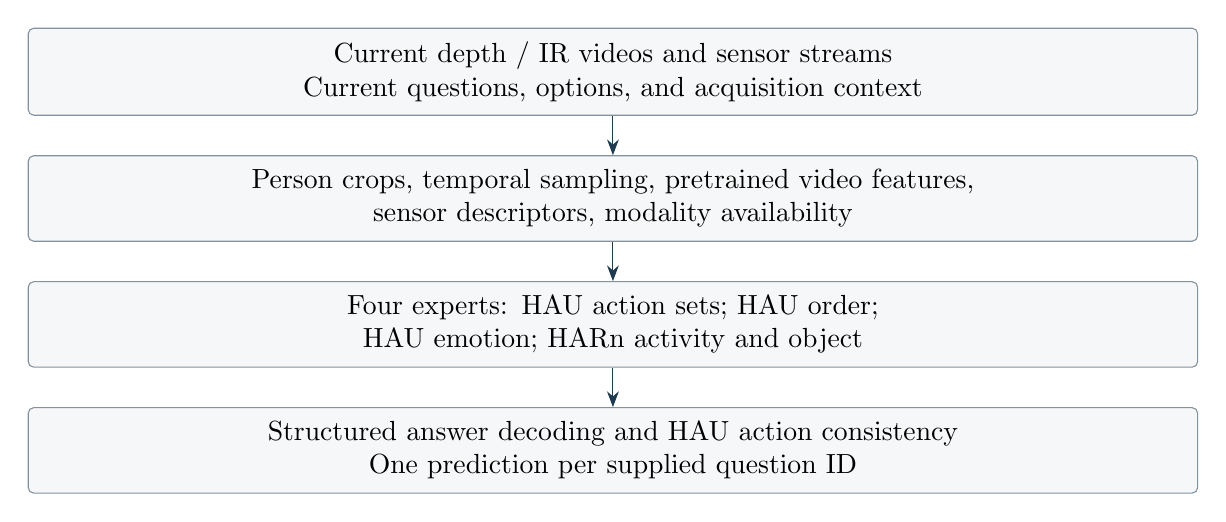
\begin{tikzpicture}[node distance=5mm,box/.style={draw=ink!55,rounded corners=2pt,fill=ink!4,align=center,text width=145mm,inner sep=5pt},arr/.style={-{Stealth[length=2mm]},draw=ink}]
\node[box] (in) {Current depth / IR videos and sensor streams\\Current questions, options, and acquisition context};
\node[box,below=of in] (f) {Person crops, temporal sampling, pretrained video features,\\sensor descriptors, modality availability};
\node[box,below=of f] (e) {Four experts: HAU action sets; HAU order;\\HAU emotion; HARn activity and object};
\node[box,below=of e] (o) {Structured answer decoding and HAU action consistency\\One prediction per supplied question ID};
\draw[arr] (in)--(f);\draw[arr] (f)--(e);\draw[arr] (e)--(o);
\end{tikzpicture}
\end{center}
\textbf{Figure 1.} Frozen primary pipeline. Context is an input to the decision stages; it is not inferred from the final prediction CSV.

The loader reads the supplied QA table and finds the corresponding visual and sensor files. It computes current-input features, routes questions by source and category, and invokes the relevant experts. HARn action probabilities are mapped to answer options, including action--object associations. HAU branches estimate action occurrence, temporal order, and emotion assignments. The final consistency stage updates HAU action answers while preserving the other task-specific outputs.

Two forms of context enter the selected method: questions referring to the same recording, and three repeated recordings belonging to a published HAU acquisition. The frozen entry recovers the latter from the published consecutive-recording convention or reads an explicit \file{acquisition.csv}. Cross-recording action evidence, emotion reasoning, temporal pooling, and group-aware option features use this relation. Thus, one output per QA row does not imply that every row is inferred in isolation.

\pageheading{3. Modalities and Model Design}
\subsection*{3.1 Modalities used}
\begin{tabularx}{\linewidth}{@{}L{22mm}L{12mm}Y@{}}
\toprule
Modality & Used & Representation and role\\
\midrule
Depth & Yes & Depth / Depth\_Color video tensors; pretrained spatiotemporal features for action and motion.\\
Infrared & Yes & Person-localized video; complementary visual evidence and crop detection.\\
Skeleton & Yes & Pose, displacement, temporal and spectral statistics; action and emotion evidence.\\
IMU & Yes & Wearable-stream statistics, dynamics and spectral descriptors; motion-sensitive emotion evidence.\\
mmWave & Yes & Point-cloud position, velocity and frame statistics; complementary motion descriptors.\\
Thermal & No & N/A; not consumed by the selected inference path.\\
RGB & No$^*$ & No challenge RGB input. $^*$External RGB training is disclosed in Section 4.\\
\bottomrule
\end{tabularx}

\subsection*{3.2 Architecture and fusion}
The visual families are R(2+1)D-18, R(2+1)D-34~\cite{r2plus1d}, and VideoMAE Base~\cite{videomae}. The released K-KUNO ensemble~\cite{kuno} supplies HAU action and temporal evidence. Our own Charades-trained R34 adds a separate action-presence signal; it replaces one calibrated-presence input, rather than replacing the entire K-KUNO-dependent system.

HARn uses equal weighting across the R18, R34 and VideoMAE visual families; the R18 family retains a two-seed average. Available views/families are combined using their masks. Skeleton evidence and action--object constraints participate in the retained downstream decoder. HAU action prediction combines visual presence, skeleton and option-context evidence before structured decoding.

Emotion inference combines a context predictor with a supervised current-recording network. This network encodes sensor and generic video descriptors into a 64-dimensional media representation and scores question/option text using deterministic hashed features. Its legal-group assignment distribution is mixed equally with the context distribution. Fusion therefore occurs at several levels: feature fusion inside specialists, probability fusion across experts, and logical consistency at the answer level.

\pageheading{4. Data Sources and How They Are Used}
\subsection*{4.1 Data source usage}
\begin{tabularx}{\linewidth}{@{}L{35mm}L{25mm}Y@{}}
\toprule
Source / type & Scope & Use in the final system\\
\midrule
Official CUHK-X / challenge data & Training and inference & Training media/labels fit heads, priors and decoders. Test media and label-free QA supply current evidence/context.\\
Charades / external data & Training only & Primary: 625 Training videos. Secondary: also 2,000 Training records (1,997 unique media).\\
K-KUNO / public competition checkpoint & Fixed inference weights & Released R34 ensemble for HAU action/sequence evidence; externally trained, not our from-scratch model.\\
Kinetics-400; IG65M / pretrained knowledge & Initialization and features & R18 Kinetics initialization; R34 IG65M then Kinetics initialization~\cite{ig65m}. No direct collection of these pretraining datasets.\\
Something-Something V2 / pretrained knowledge & Fixed encoder & VideoMAE Base checkpoint and processor; custom downstream HARn readout.\\
YOLO11n~\cite{yolo} / pretrained model & Preprocessing & Person detection for video crops.\\
Video Depth Anything Small~\cite{vda} / synthetic source & Secondary training only & Generates depth from external Charades RGB for paired-source transfer. Not loaded during submitted inference.\\
\bottomrule
\end{tabularx}

\subsection*{4.2 Selection and indirect use}
The 625-video Charades subset~\cite{charades} covers 211 people and 157 action labels, balancing people and source-class coverage without target-error selection. Invalid class intervals are masked; valid intervals are intersected with decoded video time. Source training uses action-occupancy supervision. The secondary pairs RGB with generated depth, adding cosine alignment to an RGB teacher before target adaptation. Both selected systems consume non-RGB challenge media at inference.

Historical development also used Codex-generated Test pseudo-labels in separate research and auxiliary agreement checks. No pseudo-label-fitted model is deployed in either Selected solution. The later agreement check tied the current candidates. No teacher API, retrieved answer bank, or Test ground-truth label is an inference dependency.

\pageheading{5. Training, Validation, and Expected Generalization}
\subsection*{5.1 Input construction and preprocessing}
The entry reads \file{test_qa.csv} with IDs, source, media path, category, question, and options. It locates the published visual Testing tree and the IMU/radar/skeleton Testing tree. The supplied QA table determines the workload; 682 is the original Test size, not a hard-coded inference limit. \file{sample_submission.csv} is optional.

\begin{tabularx}{\linewidth}{@{}L{36mm}Y@{}}
\toprule
Visual stream & Fixed sampling and representation\\
\midrule
K-KUNO HAU evidence & 8 windows of 2.5 s and 16 windows of 1.25 s; 16 sampled frames per window. \\
Primary source R34 & 8 windows of 2.5 s; 32 frames per window; Depth\_Color and IR; 512-dimensional pooled features per window/view.\\
Generic R18 & 16 frames; Depth and IR. HAU descriptors use 8 windows of 2.5 s. HARn retains middle features for its trained tail.\\
Generic R34 / HARn & 32 uniformly sampled frames over the recording, with retained middle features and trained tail.\\
VideoMAE / HARn & 16 uniformly sampled whole-recording frames per available view; bundled processor and pretrained encoder.\\
\bottomrule
\end{tabularx}

R18/R34 preprocessing applies the stored person ROI, resizes to $171\times128$, and center-crops to $112\times112$. Intensities are divided by 255 and standardized using mean $(0.43216,0.394666,0.37645)$ and standard deviation $(0.22803,0.22145,0.216989)$. IR is represented with the producer's prescribed channel conversion; the source R34 replicates grayscale IR across three channels. VideoMAE uses its own 224-pixel processor with ImageNet mean/std.

Frame sampling uses each video's actual frame count and frame rate; short inputs may repeat sampled indices. Window timestamps and availability masks are retained. Visual alignment is checked to a one-frame tolerance, without learned clock correction. Skeleton action descriptors use 16/32/48-frame windows. Sensors use the bundled temporal/statistical extractors rather than text prompts. Missing observations receive the saved missing-data representation and masks; no substitute modality is fabricated.

\subsection*{5.2 Training and validation protocol}
Custom components are trained on official Training subjects user1--9 and user16--24. Downstream model development uses leave-one-person-out evaluation, with subject-separated inner folds where the component selects a decoder or fusion setting. Final custom models fit their full Training scope and are frozen before Test inference. No test-time fitting is performed.

For the primary source branch, external Charades training updates R34 layers 3--4 and a source head while retaining fixed batch-normalization running statistics. The target HAU presence readout consumes 8-window, two-view, 512-channel features. Its retained recipe uses 128 hidden units, dropout 0.1, 40 epochs, learning rate $10^{-3}$, weight decay 0.01, batch size 32, and seed 20260905. Three inner folds select among fixed presence/option decoding recipes; the final readout fits all 18 Training people. Training scope and exact estimator settings accompany the saved model.

\begin{tabularx}{\linewidth}{@{}L{60mm}Y@{}}
\toprule
Validation item & Primary result / interpretation\\
\midrule
Local split & Cross-subject, 18 downstream leave-one-person-out folds.\\
Held-out subjects & Each of user1--9 and user16--24 in turn.\\
Held-out environment & N/A; no separate environment-held-out result.\\
Local complete-system result & 3914/4087 = 95.77\%.\\
Public / Private leaderboard & 94.444\% / 90.294\%.\\
Local minus Public / Private & 1.32 / 5.47 percentage points.\\
Unseen subjects / environments & No additional measured accuracy beyond the leaderboard; no numerical forecast.\\
Most consequential shift & Acquisition structure and available QA context, as well as sensor/view and activity-distribution shifts.\\
\bottomrule
\end{tabularx}

Local counts are historical downstream comparisons. These 18 people were examined repeatedly during development, and K-KUNO's complete upstream training-person roster is unavailable. Accordingly, we do not present the local percentage as a uniformly subject-excluded end-to-end benchmark. Subject-scoped heads and priors support comparison of downstream choices; the frozen Private score supplies the separate competition result.

\pageheading{6. Results and Evidence}
\subsection*{6.1 Official results and task breakdown}
\begin{tabularx}{\linewidth}{@{}Yrrr@{}}
\toprule
Selected system & ID & Public & Private\\
\midrule
Primary: source HAU + D10 & 56239668 & 0.94444 & \textbf{0.90294}\\
Secondary: target fusion + residual & 56258762 & 0.94444 & 0.90000\\
\bottomrule
\end{tabularx}

The primary is the verification target because it has the higher Private score among the two Selected submissions. The secondary adds a paired-source adapted HARn encoder, option-space fusion, and a fixed temporal residual. These additions belong to that second submitted system; they are not attributed to the primary result.

\begin{tabularx}{\linewidth}{@{}Yrrr@{}}
\toprule
Primary local question family & Questions & Correct & Accuracy\\
\midrule
HARn activity & 429 & 402 & 93.71\%\\
HARn object interaction & 133 & 128 & 96.24\%\\
HAU single action & 809 & 809 & 100.00\%\\
HAU multiple actions & 809 & 792 & 97.90\%\\
HAU combination & 790 & 788 & 99.75\%\\
HAU emotion & 809 & 752 & 92.95\%\\
HAU sequence & 308 & 243 & 78.90\%\\
\midrule
Total & 4087 & 3914 & 95.77\%\\
\bottomrule
\end{tabularx}

These counts are recomputed from archived predictions and official Training answers; they follow the protocol in Section 5.2. The decomposition identifies temporal order as a distinct source of residual error. Of 65 sequence errors, 62 occur where all related action QA answers are correct. Correct action-set answers therefore do not establish that the temporal evidence distinguishes the event order.

The secondary reaches 3919/4087 locally but does not improve the Private score. The two evaluation settings therefore support different rankings. Matched interventions below isolate component effects within the local protocol.

\subsection*{6.2 Action-set-conditioned temporal reasoning}
For four candidate actions $C$, the temporal branch scores the 24 permutations $\Pi(C)$. Let $b(\pi)\in\{0,1\}^6$ encode their pair orientations, $p$ denote predicted pair probabilities, and $\ell$ denote training-derived pair-prior logits. The baseline score, omitting permutation-independent terms, is
\[
S_0(\pi)=\bigl(\operatorname{logit}(p)+\ell\bigr)^\top b(\pi).
\]
For a supported four-action set, D9 replaces the generic order prior with a smoothed contextual distribution. Let $n_C(\pi)$ be training counts, $N_C=\sum_\pi n_C(\pi)$, and $q(\pi)=\operatorname{softmax}_{\pi}(\ell^\top b(\pi))$. Then
\[
\widetilde q_C(\pi)=\frac{n_C(\pi)+3q(\pi)}{N_C+3},\qquad
S_4(\pi)=\operatorname{logit}(p)^\top b(\pi)+\log\widetilde q_C(\pi).
\]
Counts are balanced so a repeated acquisition contributes unit mass to each observed context. D10 adds a fallback when the full four-action set has no support: for each supported three-action subset $T$, marginalize $q$ to $q_T$ and smooth its empirical counts in the same way. Decoding uses
\[
S_{10}(\pi)=S_0(\pi)+\frac14\sum_{T:N_T>0}
\left[\log\widetilde q_T(\pi|_T)-\log q_T(\pi|_T)\right].
\]
If neither support level is available, the baseline is unchanged. Here a three-action subset is a subset of the question's action vocabulary, distinct from a three-recording acquisition group.

\begin{tabularx}{\linewidth}{@{}Yrr@{}}
\toprule
Matched temporal component & Sequence / 308 & Full / 4087\\
\midrule
Pairwise baseline & 240 & 3906\\
Four-action context (D9) & 242 & 3908\\
Four-action + subset fallback (D10) & \textbf{243} & \textbf{3909}\\
\bottomrule
\end{tabularx}

The hierarchy corrects three sequence answers with no newly incorrect answer in this comparison. Four-action support accounts for two corrections; three-action fallback accounts for one. The 56 queries without either support level retain 38 correct answers. This matched experiment precedes the source-presence replacement; the primary retains its D10 temporal predictions unchanged.

\subsection*{6.3 External action evidence and consistent decoding}
The Charades-trained source encoder consumes depth-color and infrared videos for the challenge. A frozen HAU head converts its window features into 40 action-presence probabilities. These replace the calibrated-presence input of the existing joint action decoder. Other evidence sources and its decision policy remain fixed, enabling a complete-system comparison.

\begin{tabularx}{\linewidth}{@{}Yrrr@{}}
\toprule
Calibrated-presence replacement & Correct / 4087 & Fixes & Harms\\
\midrule
Retained D10 system & 3909 & -- & --\\
Generic R34 & 3912 & 7 & 4\\
Charades RGB source (primary) & \textbf{3914} & 8 & 3\\
Charades synthetic-depth source & 3911 & 7 & 5\\
\bottomrule
\end{tabularx}

Fixes and harms are relative to the retained D10 system. The RGB-source replacement improves complete-system answers by five. The effect is small and its historical subject-bootstrap interval includes zero; it supports the retained empirical choice without establishing universal superiority of RGB over synthetic-depth training. The corresponding complete submission moves Public accuracy from 0.93859 to 0.94444. Synthetic-depth paired transfer remains part of the secondary, not the primary.

\textbf{Answer consistency.} Action options are represented as atoms; a combination option is a conjunction. Single and combination questions require one option, and multiple-action questions require a nonempty set. Sequence questions supply action-presence constraints, while their ordering is handled by D10. For legal state $z$, the final decoder first minimizes changed whole-question answers:
\[
d(z)=\sum_q\mathbf{1}\{y_q(z)\neq\widehat y_q\}.
\]
Among states with minimum $d$, it maximizes the Bernoulli log score of option bits using the mean probabilities of three saved frequency models. Stable enumeration resolves exact ties. This separates admissibility from preference: constraints define compatible answers, while learned evidence selects among equally small repairs. Consistent expert answers can pass through unchanged.

\textbf{Emotion evidence.} The supervised local scorer induces a normalized probability over the same legal group assignments as the context model. Their fixed 50:50 mixture selects the final assignment. This uses actual recording/question evidence while retaining the published acquisition constraints; it is not a free-form language-model response.

\pageheading{7. Efficiency and Reproducibility}
\subsection*{7.1 Measured inference and training scope}
\begin{tabularx}{\linewidth}{@{}Yrr@{}}
\toprule
Full original Test, fresh runs & Primary & Secondary\\
\midrule
RTX 3060 Laptop GPU, 6 GB & 2043.5 s & 2134.6 s\\
Minutes for 682 questions & 34.1 & 35.6\\
Amortized seconds per QA row & 3.00 & 3.13\\
Exact original CSV reproduction & 682/682 & 682/682\\
Offline Docker execution & Yes & Yes\\
\bottomrule
\end{tabularx}

Both runs started from fresh working directories and recomputed features from original Test media. The secondary did not reuse the primary's features. No host code, Training data or precomputed feature cache was mounted. The reference CSVs are used for comparison, not as prediction inputs. The reported per-row times are batch averages with shared video processing, not single-query latency measurements.

During the primary run, sampled whole-device GPU memory peaked at 3729 MiB and sampled container memory at 8.27 GiB. The secondary finished successfully, but its separate memory monitor failed; no secondary memory peak is claimed. A supplementary RTX 4090 native run completed the primary in 1113.4 seconds. The rented 4090 did not support Docker, so it is not the container-validation platform.

Training used the local RTX 3060 Laptop, a rented RTX 4090 24 GB, and CPU workers for classifiers and structured components. Total training GPU-hours and financial cost were not aggregated across the research history and are reported as N/A. Reproduction requires frozen inference, not re-execution of all development experiments.

\subsection*{7.2 Frozen artifacts}
The committee has been given the private verification archive \file{large_KURONAME_verification_v1.zip} (2.45 GB) and the tested image archive \file{KURONAME_Docker_3060.tar.gz} (6.74 GB). The ZIP contains code, training sources, weights, configuration, Selected CSVs, the signed declaration and validation records; the image supplies the runtime. Public code/weight URL: N/A; use the previously submitted private link. The editable source accompanying this report is \file{KURONAME_Technical_Report_Source.zip}.

\subsection*{7.3 Reproduction procedure and configuration}
Download the two verification artifacts first. On a Linux x86\_64 host with NVIDIA Container Toolkit, load the tested image and mount the supplied Test data read-only:
\begin{quote}\ttfamily\raggedright
docker load -i KURONAME\_Docker\_3060.tar.gz\par
docker run -{}-rm -{}-gpus all -{}-network none \textbackslash\par
\quad -{}-shm-size 16g \textbackslash\par
\quad -v /path/to/test:/input:ro \textbackslash\par
\quad -v /path/to/output:/output \textbackslash\par
\quad kuroname:selection-3060-v1 \textbackslash\par
\quad bash inference.sh /input /output/primary.csv
\end{quote}
The archive README contains the copyable shell commands. The optional third argument \file{56258762} selects the secondary. Use a new output filename; stage logs and intermediates are retained in \file{<output_csv>.work/}. Reserve 15 GB of writable working space beyond inputs and installed artifacts.

Primary settings are in \file{configs/submission_56239668.json}; the shared component map is \file{core/conditioned_package.json}. \file{TRAINING.md}, \file{training_configs/}, and component descriptors preserve fitted recipes and seeds. D10 uses fixed contextual smoothing 3 and subset exponent 0.25. Inference fixes \file{PYTHONHASHSEED=0}, thread counts, evaluation mode, and the CUBLAS workspace convention; each producer retains its FP16/BF16/FP32 behavior.

The tested image uses Python 3.12.3, PyTorch 2.11.0+cu128, torchvision 0.26.0+cu128 and CUDA 12.8; the local host driver was 576.80. One Ampere-or-newer GPU is the intended platform. No closed-source API, runtime download, tensor parallelism or custom CUDA extension is required. The exact exported image fixes system libraries as well as Python packages.

\section*{8. Large Model Track Details}
The final system is an ensemble of open-weight video encoders and fitted specialists, not a single generative language model. A single base-model parameter count is therefore N/A; encoder identities are given in Sections 3--4 and the bundled manifest. Non-RGB videos become normalized video tensors, and sensors become numeric descriptors. The method uses feature extraction, supervised adaptation and structured decoding; prompting and token cost are N/A. Its outputs are constrained to the provided answer space.

\pageheading{9. Generalization, Limitations, and Lessons}
\textbf{Available context defines the inference problem.} The selected system uses same-recording questions and the published three-recording acquisition relation. The latter is recovered from published numbering or explicit metadata. These relations are distinct: anonymous recordings do not automatically form valid triplets. When its group assumptions fail, the original entry can reject an input or infer an incorrect group.

\textbf{Next research priorities.} The 62 sequence errors with correct related action answers motivate order-sensitive supervision rather than further increases in action-set confidence. Recording-independent context modeling is the other priority. Generated depth is not sensor-equivalent measured depth, so external transfer should be judged through full-chain comparisons after option mapping and consistency decoding.

\textbf{Post-public-phase changes.} Packaging relocated assets, added supplied-path discovery, and validated predictions in Docker; selected weights and decision settings were retained. This report introduces no new scored model.

\textbf{Conclusion.} Specialized non-RGB perception, transferred action evidence and structured decoding yield 0.90294 Private accuracy with exact offline original-Test reproduction on a 6 GB laptop GPU. The component comparisons connect these mechanisms to complete-system effects; the explicit input contract states the context required to reproduce them.

\newpage
\pageheading{10. References}
\begingroup
\renewcommand{\section}[2]{}
\begin{thebibliography}{9}
\setlength{\itemsep}{5pt}
\bibitem{cuhkx} Siyang Jiang, Mu Yuan, Xiang Ji, Bufang Yang, Zeyu Liu, Lilin Xu, Yang Li, Yuting He, Liran Dong, Wenrui Lu, Zhenyu Yan, Xiaofan Jiang, Wei Gao, Hongkai Chen, and Guoliang Xing. A Large-Scale Multimodal Dataset and Benchmarks for Human Activity Scene Understanding and Reasoning. \emph{MobiSys}, pp. 352--370, 2026. \href{https://doi.org/10.1145/3745756.3809209}{doi:10.1145/3745756.3809209}.
\bibitem{r2plus1d} Du Tran, Heng Wang, Lorenzo Torresani, Jamie Ray, Yann LeCun, and Manohar Paluri. A Closer Look at Spatiotemporal Convolutions for Action Recognition. \emph{CVPR}, 2018. \url{https://arxiv.org/abs/1711.11248}.
\bibitem{videomae} Zhan Tong, Yibing Song, Jue Wang, and Limin Wang. VideoMAE: Masked Autoencoders Are Data-Efficient Learners for Self-Supervised Video Pre-Training. \emph{NeurIPS}, 2022. \url{https://arxiv.org/abs/2203.12602}.
\bibitem{charades} Gunnar A. Sigurdsson, G\"ul Varol, Xiaolong Wang, Ali Farhadi, Ivan Laptev, and Abhinav Gupta. Hollywood in Homes: Crowdsourcing Data Collection for Activity Understanding. \emph{ECCV}, 2016. \url{https://prior.allenai.org/projects/charades}.
\bibitem{kuno} phuongncn. K-KUNO LB 0.711 R2Plus1D Model. Public Kaggle competition checkpoint. \url{https://www.kaggle.com/datasets/phuongncn/k-kuno-lb-0-711-r2plus1d-model}.
\bibitem{ig65m} moabitcoin. IG65M PyTorch: R(2+1)D-34, 32-frame, Kinetics fine-tuned release. \url{https://github.com/moabitcoin/ig65m-pytorch}.
\bibitem{vda} Depth Anything authors. Video Depth Anything Small. Training-only synthetic-depth generator, revision \texttt{256875362cff76724b920335dfb4b29dd611f66e}. \url{https://huggingface.co/depth-anything/Video-Depth-Anything-Small}.
\bibitem{yolo} Ultralytics. YOLO11. Person-detection model and software. \url{https://docs.ultralytics.com/models/yolo11/}.
\end{thebibliography}
\endgroup
\end{document}
